\documentclass[a4paper,11pt]{article}
\usepackage{dcolumn}
\usepackage{hyperref}
\usepackage{graphicx}


%opening
\title{Bayesian Econometrics - Assignment 1}
\author{James Savage}


\begin{document}


\maketitle

\section*{Note}
All programs used in this assignment are available on my \href{<www.github.com/khakieconomics>}{github repository}. Where possible, I have double-checked my answers in R, and these programs are up there too. Each section contains a link to the relevant program.



\section*{Question 1}

\subsection*{Part a) i}

The following pseudocode describes how to sample from a (lower) truncated normal distribution. 

\begin{verbatim}
input: number of draws; 
the mean of the un-truncated distribution; 
the variance of the un-truncated distribution; 
the truncation point


1. draw #of draws from (0,1) uniform distribution

2. for each draw, find the value of the inverse 
    cdf of the target truncated normal 
    distribution

\end{verbatim}

\subsection*{Part a) ii}

The function may be found here:
\url{https://github.com/khakieconomics/homework/blob/master/Bayesian_econometrics/rnormtrunc.m}

Work for the rest of question 1 using the function can be found here:
\url{https://github.com/khakieconomics/homework/blob/master/Bayesian_econometrics/question1.m}

Sense-checking using R can be found here:
\url{https://github.com/khakieconomics/homework/blob/master/Bayesian_econometrics/Question_1.R}

\subsection*{Part b)}

A KDE plot of the draws is given. 

\begin{figure}
  \centering
  % Requires \usepackage{graphicx}
  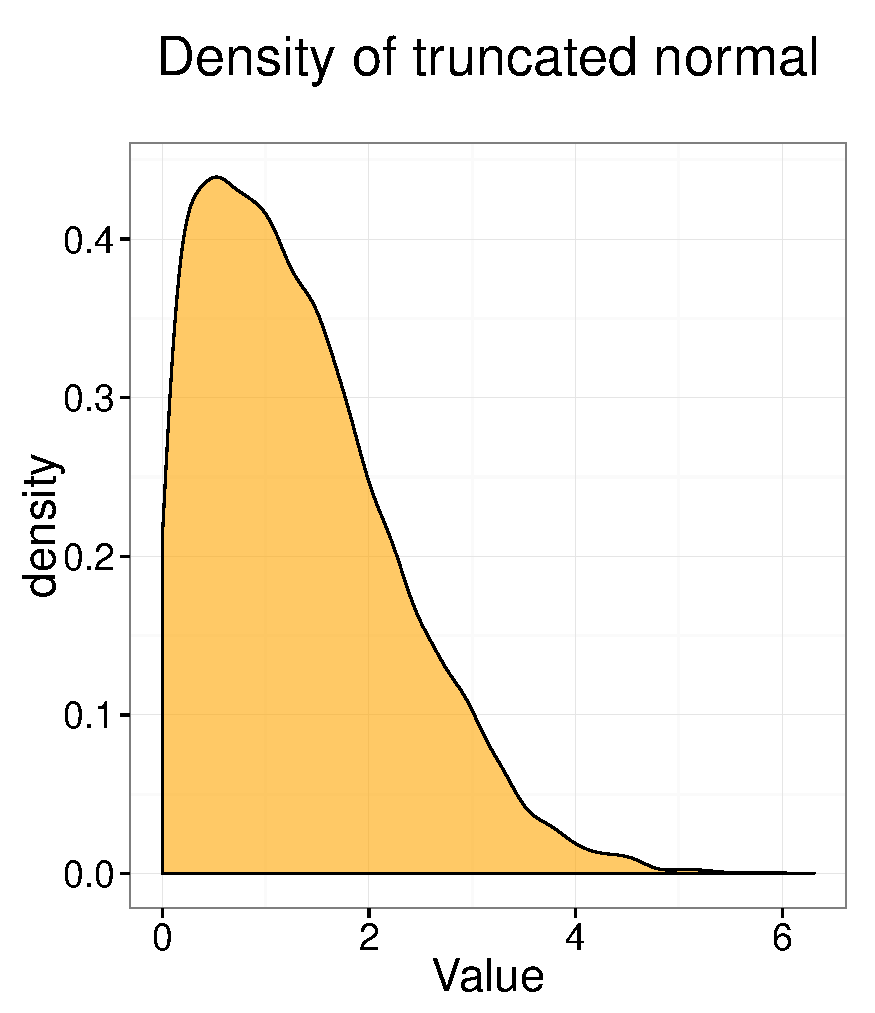
\includegraphics[width=300pt]{truncated_density.pdf}\\
  \label{density}
\end{figure}


\subsection*{Part c) i}

To find the probability that the parameter $\theta$ lies between 0 and 1, all we need to do is find the proportion of draws from the distribution that are between 0 and 1.

\begin{verbatim}
  mean(draws>0 & draws<1)
\end{verbatim}

\noindent Which gives us $0.419$.

\subsection*{Part c) ii)}

The 0.05 and 0.95 quantiles of the distribution are $[0.13, 3.12]$, which has a length of a little less than 3 (2.99).

\subsection*{Part d)}

Given the distribution has a lot of mass at the truncation point, a 90 per cent credibility interval could probably contain that point. The $[0, 0.9]$ quantile interval, $[0, 2.65]$, is shorter, at only 2.65---a significant reduction.
\end{document}

 